\section{Protocol specifications and speed comparisons}
In this section we compare the specifics of implementations of $\mathrm{BCNS}$ and $\mathrm{NewHope}$. In particular, generation of shared polynomial and polynomial multiplication algorithm. They are both important as they directly impact the bandwidth and speed of key-exchange.

\subsection{Sending shared polynomial, two fundamentally different approaches}
Shared polynomial is specially important as it needs to be shared with other party to enable key-exchange. Typically, the file size of this polynomial is relatively large as it should be generated from a uniform distribution (i.e. unlike error or noise polynomial, no upper-bound should be applies to it's coefficients). The following table shows the size of shared polynomial in Kilobytes for BCNS and NewHope protocols:

\begin{table}[H]
\centering
\begin{tabular}{|l|l|l|l|l|}
\hline
Protocol            & Number of coefficients & Modulus & Size of shared polynomial                 & Payload                \\ \hline
$\mathrm{BCNS}$     & 1024 & $2^{32} - 1$    & $ 1024 \times 32 \text{bits} \approx 4 \text{KB}$     & $\approx 4 \text{KB}$  \\ \hline
$\mathrm{NewHope}$  & 1024 & $12289$         & $ 1024 \times 14 \text{bits} \approx 1.8 \text{KB}$   & $256$-bit seed         \\ \hline
\end{tabular}
\caption{Maximum size of shared polynomial and payload}
\end{table}

$\mathrm{BCNS}$ during install (or build) of Open-$\mathrm{SSL}$ will generate a uniformly random shared polynomial and will use it for all the key-exchanges. Reusing shared polynomial more than once is completely fine under Ring-$\mathrm{LWE}$ hardness assumption. But the downside is key-exchange initiator also needs to send the shared polynomial to other party and sending $4\text{KB}$ of data is not an ideal solution. $\mathrm{NewHope}$ protocol addresses the issue by sending a \textit{seed} so that other party can recreate the shared polynomial by themselves instead. In details, $\mathrm{NewHope}$ uses $256$-bit seed through $\mathrm{SHAKE}\text{-}128$ which is a hash function with arbitrary length output. Then slicing the resulting $16384$ bits into $1024 \times 16\text{ bit}$ numbers. Each of those integers is reduced to modulo $2^{14}$ (i.e. the two most-significant bits are set to zero) and then used as a coefficient of shared polynomial if it is smaller than $q$ and rejected otherwise (or $0$ is used instead).

The advantage that can be observed here is that some of the coefficients of shared polynomial would be set to $0$ hence shared polynomial would not be too large and not too small. Therefore, in polynomial multiplication, we would not be dealing with a polynomial with relatively large coefficients, this results in a increased speed in key-exchange.

The following is a demonstration of creating a uniformly random polynomial from a random seed and extracting polynomial coefficients from it:


\begin{algorithm}[H]
    \caption{Extracting coefficients of shared polynomial as described in $\mathrm{NewHope}$}
    \begin{algorithmic}[1]
        \State modulus $\leftarrow$ 12289
        \State number\_of\_coefficients $\leftarrow$ 1024
        \item[]
        \Function{create\_coefficient\_array}{seed}
            \State \Comment{set the seed and length of output in bits}
            \State raw $\leftarrow$ SHAKE-128(seed, number\_of\_coefficients $\times 16$) 
            \State chunks $\leftarrow$ convert hex digest of `raw' to chunks (or sub-strings) of bit length $= 16$
            \For{$i \gets 0 \text{ to } \text{length(chunks)}$}
                \State \Comment{reduce chunk to modulo $2^{14}$ by setting 2 significant bits to zero}
                \State chunks[$i$] $\leftarrow$ chunk[$i$] XOR 0xC000
                \State \Comment{if coefficient is greater than modulus then set to 0}
                \State chunks[$i$] $\leftarrow$ 0 if chunk[$i$] $\ge$ modulus else chunks[$i$] 
            \EndFor
            \Return chunks
        \EndFunction
        \item[] \Comment{set the seed and then extract coefficients}
        \State seed $\leftarrow$ 256 bit sampled uniformly random
        \State coefficients $\leftarrow$ create\_coefficient\_array(seed)
    \end{algorithmic}
\end{algorithm}

\iftoggle{verylong}{
\lstinputlisting[language=Python, caption=Extracting coefficients of shared polynomial as described in $\mathrm{NewHope}$ protocol using SageMath]{code_snippets/newhope_uniform_sampler.sage}
}{}

\iftoggle{verylong}{
\lstinputlisting[language=Python, caption=Plot of number of non-zero coefficients as a result of NewHope's shared polynomial generation algorithm using SageMath]{code_snippets/analysis_of_shared_polynomial.sage}
}{}



In the following bar chart plot we can see that number of non-zero coefficients of shared polynomial is on-average $200$ out of all $1024$ coefficients. This is good as it makes the shared polynomial sufficiently large, not too small, but still uniformly at random.

\begin{figure}[H]
    \centering
    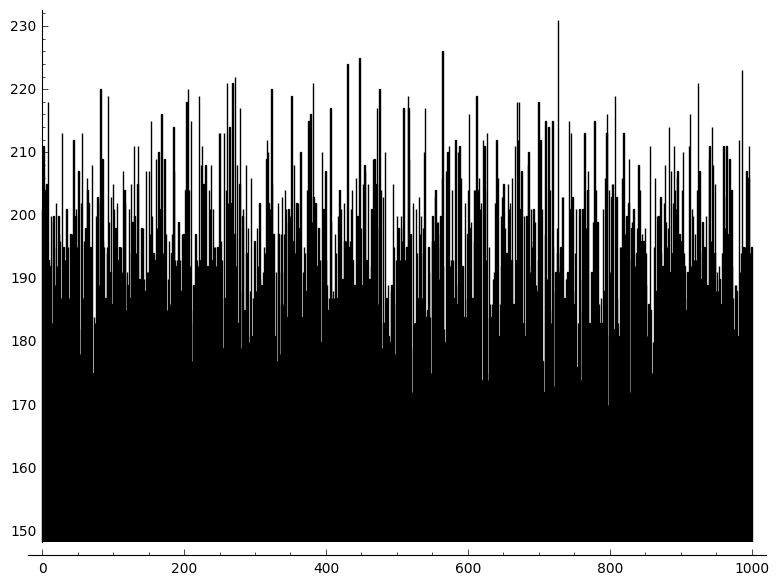
\includegraphics[scale=0.4]{shake_distribution}
    \caption{Plot of number of non-zero coefficients after creating $1000$ shared polynomials}
\end{figure}


\iftoggle{verylong}{
\subsection{Polynomial multiplication algorithm}
$\mathrm{BCNS}$ protocol uses Split-radix $\mathrm{FFT}$ algorithm which is a variant of Mersenne Number Transform ($m = 2^k - 1$) outlined by H. Nussbaumer in \cite{1163372} known. This algorithm is based on recursive negacyclic convolutions and this naturally applies to cyclotomic rings where the degree is a power of $2$. It requires to use a composite modulus. Note that $2^{32} - 1$ is not a prime as $q = (2^{1} + 1)(2^{2} + 1)(2^{4} + 1)(2^{8} + 1)(2^{16} + 1)$. This polynomial multiplication method requires $\text{O}(n \log n)$ multiplications in $\mathbb{R}$ for $n$-digit numbers.

On the other hand, $\mathrm{NewHope}$ protocol uses Schonhage-Strassen algorithm which is a variant of Fermat Number Transform ($m = 2^{2^{k}}+1$) outlined by A. Schonhage and V. Strassenin \cite{Schonhage1971}. Akim, author of $\mathrm{NewHope}$ protocol, chose $q = 12289$ as it is the smallest prime for which it holds that $q \equiv 1 (\bmod$ $2n)$ so that the number-theoretic transform ($\mathrm{NTT}$) can be realized efficiently. Note that $2n = 2^{11} \mid (q - 1) = 12288 = 2^{12} + 2^{13}$. This polynomial multiplication method requires $\text{O}(n \log(n) \log (\log(n) ))$ multiplications in $\mathbb{Z}$ for $n$-digit numbers. Alkim discussed using Nussbaumer's Split-radix $\mathrm{FFT}$ algorithm instead due to a better time complexity but the $\mathrm{C}$ implementation was not much faster than Schonhage-Strassen algorithm implementation. But he hinted it is a possibility in future implementations to switch to Nussbaumer.
}

\subsection{Performance analysis}
The following is table comparison of clock cycles of $\mathrm{BCNS}$ and $\mathrm{NewHope}$ protocols (both $\mathrm{C}$ and $\mathrm{AVX2}$ ref. codes). Clearly $\mathrm{NewHope}$ dominates the $\mathrm{BCNS}$ protocol in terms of speed and it's assembly language implementation is $\approx 4 \times$ faster than $\mathrm{C}$ ref. code. Note that $\mathrm{BCNS}$ protocol generates the shared polynomial during the install (or build) of Open-$\mathrm{SSL}$ so the numbers below for $\mathrm{BCNS}$ does not include the clock cycles of that. However, the numbers for $\mathrm{NewHope}$ includes a $\approx 37000$ clock cycles for generation of shared polynomial. But we always have an option to cache the shared polynomial indefinitely so we do not count it in clock cycles analysis but it would directly impact the required bandwidth for key-exchange. Note that Advanced Vector Extensions (AVX) are extensions to the $\mathrm{x86}$ instruction set architecture for microprocessors from Intel and AMD.

The reason for speed increase of $\mathrm{NewHope}$ is due to smaller modulus and choice of Binomial noise sampler which is more efficient to sample as oppose to Gaussian sampler. 

\begin{table}[H]
\centering
\begin{tabular}{|l|l|l|l|l|}
\hline
Protocol                    & $\mathrm{BCNS}$ & $\mathrm{NewHope}$'s $\mathrm{C}$ ref.   & $\mathrm{NewHope}$'s $\mathrm{AVX2}$ ref.  & $\mathrm{X25519}$          \\ \hline
Key generation (server)     & $ 2477958$         & $ 258246$                                             & $ 88920$        & $ 52169$  \\ \hline
Key generation (client)     & $ 3995977$         & $ 384994$                                             & $ 110986$       & $ 52169$  \\ \hline
Shared key computation      & $ 481937 $         & $ 86280 $                                             & $ 19422$        & $ 159128$ \\ \hline
Sum of clock cyles          & $ \approx6955\text{K}$    & $ \approx729\text{K}$                          & $ \approx219\text{K}$  & $ \approx263\text{K}$ \\ \hline
\end{tabular}
\caption{Clock cycle comparisons of $\mathrm{BCNS}$, $\mathrm{NewHope}$ and fastest $\mathrm{X25519}$ implementation}
\end{table}


Clearly $\mathrm{NewHope}$ is faster with regards to sum of clock cycles in comparison with state-of-the art elliptic curve cryptography based Diffie-Hellman key-exchange ($\mathrm{ECC}$). Total clock cycles of $219\text{K}$ vs. $263\text{K}$. More specifically $\mathrm{X25519}$; the fastest implementation is called Sandy2x written in 2015 by T. Chou (student of D. Bernstein) which is also written in $\mathrm{AVX2}$ assembly language \cite{cryptoeprint:2015:943}. This means that lattice based key-exchange is not only a quantum safe option but it also faster than today's key-exchange protocols.

Alkim et al. went further and provided $\mathrm{ARM}$ Cortex implementation which can be used for portable devices, because these devices usually use $\mathrm{ARM}$ architecture in contrast with $\mathrm{AVX2}$ which is primarily used in Desktop computers. The $\mathrm{ARM}$ reference implementation runs in $\approx 1.5\text{M}$ cycles in contrast with $\approx 3.6 \text{M}$ cycles of fastest $\mathrm{X25519}$ implementation in ARM.

NewHope's $\mathrm{AVX2}$ reference implementation (not the $\mathrm{C}$ implementation to make comparison fair) out performs the fastest elliptic curve based Diffie-Hellman in conjunction with either RSA or ECDSA (elliptic curve Digital Signature Algorithm), hence, it would make it easy pick to replace existing key-exchange protocol. Also, NewHope outperforms post-quantum competitors by factor of two. Below shows the speed comparison of NTRUEncrypt (or NTRU), Frodo (which is identical to $\mathrm{BCNS}$ but uses $\mathrm{LWE}$ as oppose to Ring-$\mathrm{LWE}$ variant), $\mathrm{BCNS}$ and NewHope.

\begin{figure}[H]
    \centering
    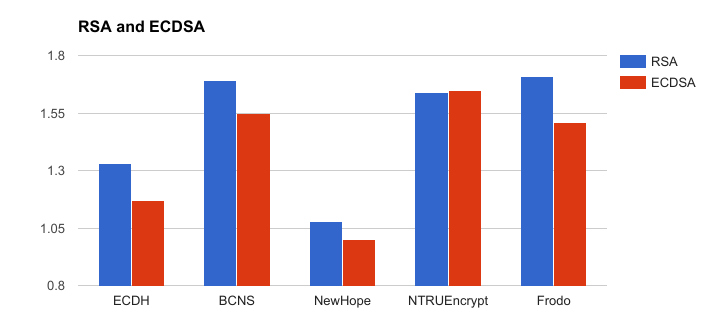
\includegraphics[scale=0.45]{performance-signature}
    \caption{TLS handshake latency (KEX protocols in conjunction with RSA and ECDSA)}
    \figuresubtitle{The shorter the bar chart, the faster TLS handshake would be.}
\end{figure}


To summarize, NewHope is a key-exchange protocol that is believed to be resistant to attacks by quantum computers but RSA and ECDSA are vulnerable. However, quantum computers are still being development and they are not available yet, so switching to NewHope would not result in any overhead, but it would also make key-exchange resistant to quantum computers and faster.

\subsection{Hybrid approach with \texorpdfstring{$\mathrm{X25519}$}{X25519}}
Authors of both $\mathrm{BCNS}$ and $\mathrm{NewHope}$ note that the Ring-$\mathrm{LWE}$ problem is hypothesised to be resistant to quantum attack, but we do not know that. In fact, we also do not know that it is resistant to attacks by classical computers. It is possible that someone will develop a classical algorithm tomorrow that breaks the scheme above. Thus Ring-$\mathrm{LWE}$ key-exchange should be used concurrently with a standard Diffie-Hellman (e.g. $\mathrm{X25519}$) and their shared key should concatenated (padded with) with each other to combine security of both future and past. Both $\mathrm{BCNS}$ and $\mathrm{NewHope}$ implementations in Open-$\mathrm{SSL}$ and Boring-$\mathrm{SSL}$ have options for hybrid key-exchange but they are set to {\lstinline[basicstyle=\ttfamily\color{black}]|false|} by default.

\subsection{Addition to popular cryptographic libraries}
Ring-$\mathrm{LWE}$-based ciphersuite described in the previous subsection are both implemented into Open-SSL and Boring-SSL. Specifically, two new ciphersuites, all designed to achieve a 128-bit security level. The two ciphersuites are: \texttt{RLWE-ECDSA-AES128-GCM-SHA256} and \texttt{RLWE-RSA-AES128-GCM-SHA256}, and they consist of:

\begin{itemize}
    \item Key-exchange based on Ring-$\mathrm{LWE}$ key exchange
    \item Authentication based on ECDSA (elliptic curve Digital Signature Algorithm) or RSA digital signatures
    \item Authenticated encryption based on AES-128 in GCM (Galois Counter Mode)
    % which provides confidentiality as well as message integrity without the addition of a separate MAC
    \item Key derivation and hashing based on SHA-256
\end{itemize}

All these ciphersuite require TLSv1.2 because of the use of AES-GCM (provides both privacy or encryption and integrity), but TLSv1.0 ciphersuites using AES in CBC mode are possible.
